\rhead{Robot Middleware}

\chapter{Robot Middleware and Controller Development}
\label{sec:robot_middleware}

\begin{figure}[!h]
\centering
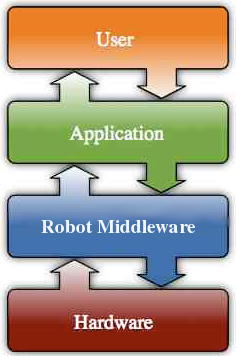
\includegraphics[width=0.5\columnwidth]{figures/3_abstraction.jpg}
\label{fig:3_abstraction}
\caption{Middleware layers.}
\end{figure}
\newpage

\begin{wrapfigure}{r}{0.55\columnwidth}

\includegraphics[width=0.53\columnwidth]{figures/3_app_store.jpg}
\end{wrapfigure}

Given a robot embodiment and a program that controls the robot, middleware serves as an abstraction between the hardware and the robot client that allows for writing robot controllers not dependent on any specific platform, as seen in Figure \ref{fig:3_abstraction}\footnote{Source: Golftheman, http://en.wikipedia.org/wiki/File:Operating\_system\_placement.svg}. The need for robot middleware arises out of the question of how to program our robots to perform desired tasks. The straightforward approach is to write and compile a program that directly sends low level commands to the robot base in order to perform the robot's ``cognitive'' functions. This one-off solution may be sufficient for programming the robot to perform one specific task on top of one specific robot platform.  However, the following challenges arise from applying this approach to robotic application development:

\begin{itemize}
\item Portability to other robot platforms or new devices.
\item Scalability to growth in functionality.
\item Reusability for other projects.
\item Interoperability between functions and languages.
\end{itemize}

To enhance the application development for robots, middleware services exist to provide an abstraction layer between computation and embodiment, similar to the hardware abstraction layer in operating systems. Middleware allows any robot controller to run on any robot platform, thus the controller software is not specific to the hardware. Between the hardware at the lowest layer and a client program at the highest layer is the middleware, which provides an interface to the robot's devices and marshals the high level commands of the client program to the low level commands understandable by the robot hardware. Middleware aims to overcome the above listed challenges by simplifying the development process, enhancing software integration and reuse, supporting interoperability, providing efficient utilization of robot components and resources, and providing interfaces that hide the low-level hardware complexity.

Although the Create platforms we are using in CS148 are relatively simple since we only need access to a handful of sensors and actuators, many robotic applications today are complex assemblages, consisting of many heterogeneous hardware components build by different manufacturers, and multiple software modules written in different languages. Given such a platform, the need for middleware is essential, allowing for modular design while coordinating the communication among the components efficiently and providing interoperability, portability and robustness.

There are several existing middleware packages for robotics, such as \href{http://code.google.com/p/lcm/}{LCM}, \href{http://www.orocos.org/}{Orocos}, \href{http://eris.liralab.it/yarp/}{YARP}, \href{http://carmen.sourceforge.net/}{CARMEN}, \href{http://msdn.microsoft.com/en-us/robotics/default.aspx}{Microsoft Robotics Studio} and JAUS. This course focuses on two: Player and the Robot Operating System, although there is mention of other middleware systems as well.

At the end of this chapter you will be able to:
\begin{itemize}
\item Understand the Player and/or ROS robot middleware system as an abstraction between the robot hardware and software.
\item Understand the basic concepts of a handful of other middleware systems.
\item Know how to send commands to and receive sensory information from the robot using either Player or ROS.
\item Write a basic robot client application to control the robot.
\end{itemize}

\section{Player/Stage/Gazebo}

\href{http://playerstage.sourceforge.net}{PSG} is a robot interface and simulation software suite that expose drivers through a simple interface for robotic applications. The core of PSG is the \href{http://playerstage.sourceforge.net/wiki/Player}{Player robot interface}, which is a framework for robot control consisting of devices, robot servers and robot clients.

\begin{figure}[!h]
\label{fig:PlayerMiddleware}
\centering
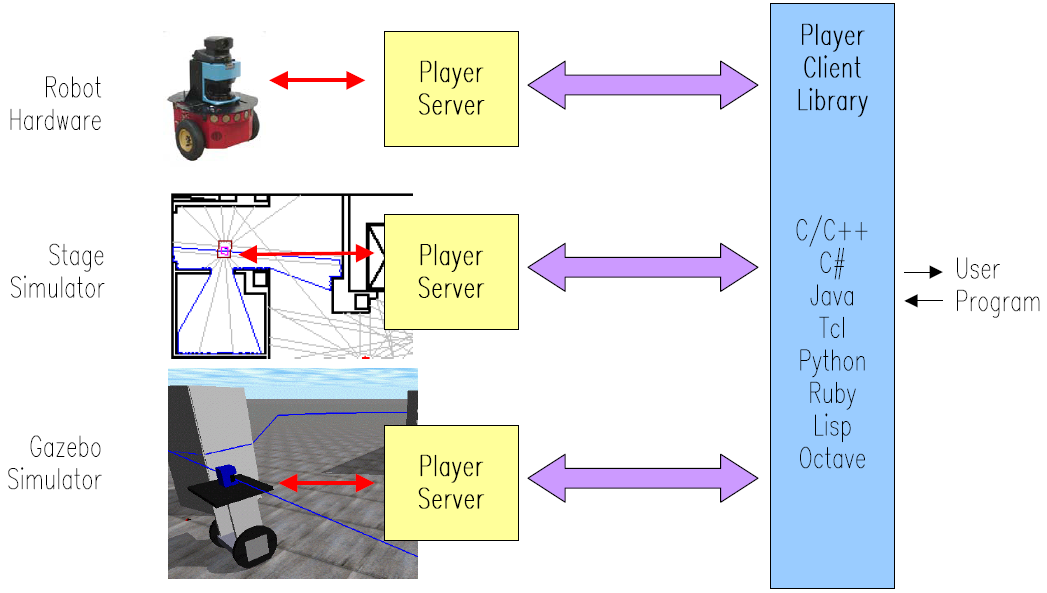
\includegraphics[width=0.8\columnwidth]{figures/3_player_abstraction.png}
\caption{Player middleware abstraction.}
\end{figure}

Running on your robot, Player provides a clean and simple interface to the robot's sensors and actuators over a TCP/IP (or UDP/IP) network. Client programs talk to Player over a TCP socket, read data from sensors, write commands to actuators, and configure devices on the fly. Figure \ref{fig:PlayerMiddleware}\footnote{Source: http://www.ki.inf.tu-dresden.de/~wiki/Robotics/Creatures/PlayerTutorial.pdf} illustrates the Player middleware abstraction between hardware and client applications.

One of the major advantages of Player as a robot server is its independence from a particular client-development language.  The interaction between Player and a client program is done completely over a TCP/IP (or UDP/IP) network connection. The communication between the Player client and Player server are illustrated in Figure \ref{fig:ClientServer}\footnote{Source: http://www.ki.inf.tu-dresden.de/~wiki/Robotics/Creatures/PlayerTutorial.pdf}.  Thus, any language with libraries that supports Player functionalities can be used to develop robot clients.  The best-supported client languages are C and C++ (supported through libplayerc and libplayerc++). Client programs can run on any machine that has a network connection to your robot and can be written in any language that supports TCP sockets. Additionally Player is designed to be platform independent; it supports a variety of robot hardware and Player's modular architecture makes it easy to add support for new hardware.

\begin{figure}[!h]
\centering
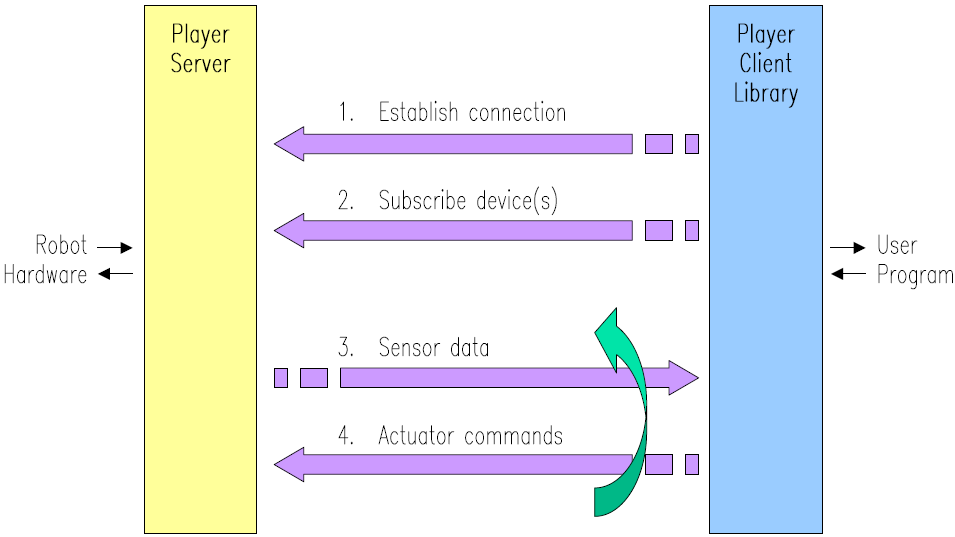
\includegraphics[height=0.45\columnwidth]{figures/3_communication.png}
\caption{\label{fig:ClientServer}Client/server communication.}
\end{figure}

Player is complemented by two simulation systems, \href{http://playerstage.sourceforge.net/wiki/Stage}{Stage} and \href{http://playerstage.sourceforge.net/wiki/Gazebo}{Gazebo}.  Stage simulates a population of mobile robots, sensors and objects in a two-dimensional bitmapped environment. Stage is designed to support multi-agent autonomous systems, so it provides fairly simple, computationally cheap models of lots of devices rather than attempting to emulate any device with great fidelity.  Gazebo is a physically simulated multi-robot simulator. Like Stage, it is capable of simulating a population of robots, sensors and objects, but does so in a physically dynamic three-dimensional world using the \href{http://www.ode.org/}{Open Dynamics Engine}. It generates both realistic sensor feedback and physically plausible interactions between objects with higher computational overhead.  These simulation systems are often an excellent means to prototype robot controllers.  However, these simulators do not have the same uncertainty and nondeterminism as faced in the real world.  We strongly recommend to students to thoroughly testing their controllers on a real robot before demoing or submitting assignments.

\subsection{Client/Server Architecture}

\begin{wrapfigure}[21]{r}{0.4\columnwidth}
\centering
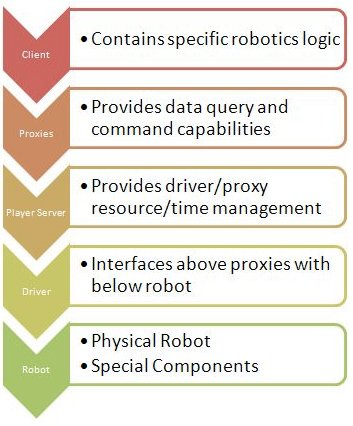
\includegraphics[height=0.5\columnwidth]{figures/3_player_model.jpg}
\caption{\label{fig:player_model}The Player model's layers of abstraction.}
\end{wrapfigure}

 
Player is a device server that provides an interface to robots, sensors and actuators. The components of the Player model is illustrated in Figure \ref{fig:player_model}\footnote{Source: http://psurobotics.org/wiki/index.php?title=Player/Stage\_Drivers}.

Devices (e.g., a laser, a camera, or a complete robot) are the actual hardware in the real world or simulated hardware that exists in a virtual environment maintained by Stage or Gazebo. Hardware resides at the lowest level in this model.

A robot server (e.g., Player) is the information interface between the robot and any program that requests information from or sends commands to the robot.  Regardless of whether a device is real or simulated, the robot server provides the same interface to the robot for client programs.  Thus, controllers developed on a simulated device will immediately run the equivalent real robot device.  (Note: A robot's {\bf behavior} is a function of both its controller and environment.  A robot controller working in one environment does not necessarily imply the same controller will yield the same behavior in new or similar environments, given PSG support for the device.)

A robot client, at the highest level in this model, is a user-developed program that accesses robot functions through the robot server.  The robot client will first establish a connection to the robot's server and then command the robot by reading data from the server and sending appropriate control command back.  The job of the developer is to write control programs that produce commands that yield desired behavior from information received from the robot server\footnote{Referring to the lecture on autonomous control, the description of the robot client should remind you of feedback control (i.e., commands [$u_t$] that produce desired state [$x_d$] given observations [$y_d$]).}  

Proxies are used by the client to retrieve information from a sensor or control an actuator; they expose interfaces to both hardware devices and existing implemented algorithms. 

Drivers reside on top of the robot and provide access to specific functions of the robot. 

Player uses a TCP socket-based client/server model, illustrated in Figure \ref{fig:ClientServer}. The client is a given robot application which interacts with the server running on the robot. The server exposes devices as proxies and publishes data continuously. The client first establishes a network connection with the robot server and subscribes to robot proxies. The client then runs in a continual loop, receiving data from and sending actuator commands to the server. Because Player follows a publish/subscribe messaging paradigm to control the robot over a network, there is no dependency on which programming language robot applications are written in\footnote{Given that the programming language has a Player client library to provide the appropriate messages, such as libplayerc for the C language.} and clients can execute from any computer on the network.
 
\subsection{Proxies}
 
The server continually publishes proxy information and the client sets variables to subscribed proxies to control the robot. The information being sent over the network between the client and server is only with respect to the proxies the client explicitly initialized. 

The proxies that are of interest to applications written in CS148:
\begin{itemize}
\item position2d: controls mobile robot bases in 2D. Client sends motor commands for velocity control by setting a forward and rotate speed to the robot; allows access to the odometric information.
\item bumper: returns data from the bumper device. This proxy accepts no commands.
\item ir: provides access to an array of infrared (IR) range sensors. The ir proxy controls two sets of ir devices on the Create. The first is a small infrared on the tip of the Create that senses virtual walls; the second set are four ir sensors on the bottom of the Create for detecting cliffs on the ground.
\item camerauvc: allows access to a USB camera and retrieves images from a camera device.
\item blobfinder: provides access to devices that detect blobs in images used for color recognition. 
\end{itemize} 

The full list of device proxies can be found \href{http://playerstage.sourceforge.net/doc/Player-cvs/player/group\_\_playerc\_\_proxies.html}{here}.

\subsection{Player Quick Start with Create}
\label{sec:player_quickstart}

The following are instructions on how to use Player as a middleware
abstraction to send commands to a robot. This is an example of client
application in C++ that controls an iRobot Create to continually
rotate in place and read bumper information from the robot.

\begin{enumerate}

\item \label{sec:3_create_client}Create a \texttt{client.cpp} program using the code below.

\begin{verbatim}
#include <stdio.h>
#include <libplayerc++/playerc++.h>
#include <signal.h>

//Use the player namespace, for cleanliness
using namespace PlayerCc;

//declare Ctrl-C-related variables
bool endnow = false;
//function to receive signals
void stopper(int x)
{
  endnow = true;
}

int main(int argc, char** argv)
{
  //Player setup
  PlayerClient *client = new PlayerClient(argv[1],6665);
  client->SetDataMode(PLAYER_DATAMODE_PULL);
  client->SetReplaceRule(true,-1,-1);

  // Create a position2d proxy (device id "position2d:0") and susbscribe
  // in read/write mode
  Position2dProxy *posProxy = new Position2dProxy(client,0);
  //set the robot to be stationary
  posProxy->SetSpeed(0,0);

  // Create a bumper proxy and subscribe
  BumperProxy *bumperProxy = new BumperProxy(client, 0);

  //tell the function 'stopper' to receive all SIGINT signals.
  signal(SIGINT,stopper);
  while(!endnow)
  {
    // read from the proxies
    client->Read();

    double forward = 0.0;
    double rotate = 0.3;
	
    printf("Forward is %g, rotate is %g.\n",forward,rotate);
    printf("Left: %d     Right: %d\n",
    bumperProxy->IsBumped(0),bumperProxy->IsBumped(1));
    // send commands to control the motors
    posProxy->SetSpeed(forward,rotate);
  }
  posProxy->SetSpeed(0,0);
		
  //cleanup
  delete posProxy;
  delete bumperProxy;		
  delete client;
		
  return 0;
}
\end{verbatim}

This program uses \texttt{libplayerc++}, which is a C++ client library for the Player server. Because libplayerc++ is used in this example, the position2d and bumper device proxies are not directly accessed. Instead the Position2dProxy and BumperProxy classes are used which control the position2d and bumper devices, respectively. Please see the \href{http://playerstage.sourceforge.net/doc/Player-cvs/player/classPlayerCc\_1\_1Position2dProxy.html}{Position2dProxy Class Reference} and the\href{http://playerstage.sourceforge.net/doc/Player-cvs/player/classPlayerCc\_1\_1BumperProxy.html}{BumperProxy Class Reference} for the public member functions of each class.

 This client first creates a PlayerClient proxy and establishes a connection to the server on the IP specified in the command-line argument (which can just be ``localhost'') listening on port 6665. PositionProxy and BumperProxy objects are created, using the client proxy object to establish access to the position2d and bumper devices. The program enters a loop (that may be exited using Ctrl-c) that spins the robot in place by sending commands to control the actuators by setting the velocity via the position2d proxy. Furthermore the client accesses the sensory information from the bumper proxy to determine if the bumper is currently pressed.

\item \label{sec:3_config_file}As described in \ref{sec:player213}, a Player configuration file must reside in a directory on the robot where you will start the Player server. Configuration files are used to inform the Player server which drivers need to be instantiated. The config file consists of driver sections, declared by the keyword \texttt{driver()}, which configure drivers. A driver section is composed of option-value pairs that are whitespace separated. Both the \texttt{name} and \texttt{provides} options are required in a driver section. The \texttt{provides} keyword specifics the device address(es) through which the driver can be accessed. The \texttt{requires} keyword specifies the device address(es) to which the driver will subscribe.

Below is a sample \texttt{create.cfg} used for this exercise:

\begin{verbatim}
driver
(
        name "create"
        provides ["position2d:0" "bumper:0" "power:0" "ir:0"]
        port "/dev/ttyUSB0"
)

driver
(
        name "camerauvc"
        provides ["camera:0"]
)

driver
(
        name "cmvision"
        provides ["blobfinder:0"]
        requires ["camera:0"]
        colorfile "colors.txt"
)
\end{verbatim}

\noindent Please refer to the \href{http://playerstage.sourceforge.net/doc/Player-1.6.5/player-html/configfile.php}{configuration files link} and the tutorial \href{http://playerstage.sourceforge.net/doc/Player-2.1.0/player/group\_\_tutorial\_\_config.html}{writing configuration files} to learn more about config files.

\item pkg-config, a tool that searches for installed libraries when compiling, must know where libplayerc++ is installed. By default the pkg-config files for Player are installed in /usr/local/lib/pkgconfig and this directory should be in the search path for pkg-config. \\
Run: \texttt{pkg-config --libs playercore}\\
If the output is similar to ``-lplayercore -lltdl -lpthread -lplayererror", you should be fine. Otherwise you will have to set the PKG\_CONFIG\_PATH environment variable to include the /usr/local/lib/pkgconfig path\footnote{Source: http://playerstage.sourceforge.net/doc/Player-2.1.0/player/install.html}:\\
\texttt{export PKG\_CONFIG\_PATH=/usr/local/lib/pkgconfig:\$PKG\_CONFIG\_PATH}

\item Compile the client application:\\
\texttt{g++ -o client `pkg-config --cflags playerc++` client.cpp `pkg-config --libs playerc++`}\\
(Best to copy and paste this line; note the above single quotes are a different ASCII character then the typical single quote and you will get a compile error if this is not correct).

\item Turn on the Create base and the EeePC.

\item Start the Player server on the robot: \texttt{player create.cfg}

\item Run the client application.
\begin{itemize}
\item If locally executing the client: \texttt{./client localhost}.
\item If the robot is on a wireless network, run the following from another computer on the network: \texttt{./client <robot IP>} where \texttt{<robot IP>} is the IP address of the robot.
\end{itemize}

\end{enumerate}

\noindent Please refer to the Player website for a simple \href{http://playerstage.sourceforge.net/doc/Player-2.1.0/player/group\_\_libplayerc\_\_example.html}{Player C example}, and also for another \href{http://playerstage.sourceforge.net/doc/Player-2.1.0/player/group\_\_cplusplus\_\_example.html}{Player C++ example}.

\section{ROS}

ROS is a robotics software framework that provides an interface to the
robot's sensors and actuators over an IP network. ROS enables a
peer-to-peer network of distributed processes that process data
together and use the ROS communication infrastructure.  According to
the system's developers:
 
\begin{quote}
\href{http://www.ros.org/wiki/ROS/StartGuide}{Robot Operating System (ROS)}, a \href{http://www.willowgarage.com/}{Willow Garage} software platform, is an open-source, meta-operating system for your robot. It provides the services you would expect from an operating system, including hardware abstraction, low-level device control, implementation of commonly-used functionality, message-passing between processes, and package management. It also provides tools and libraries for obtaining, building, writing, and running code across multiple computers. 
\end{quote}

\subsection{Peer-to-Peer Messaging Model}

%GRAPHIC OF CONTROLLED SERVER
\begin{figure}[!ht]
\centering
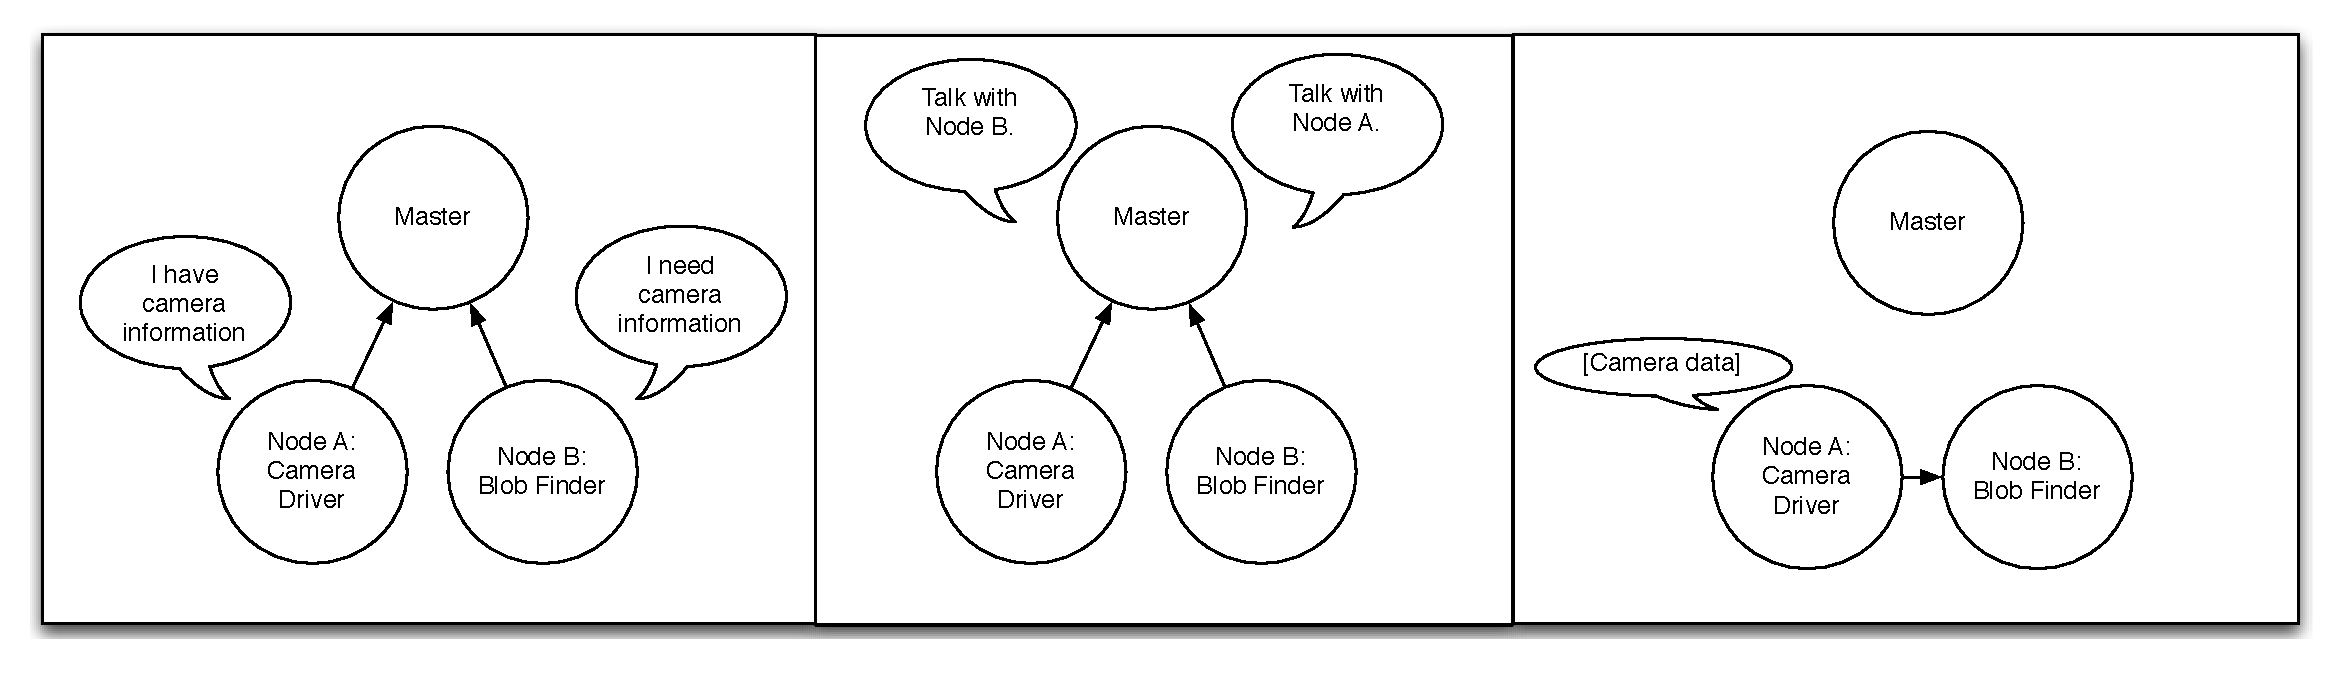
\includegraphics[width=39pc]{figures/3_rosmaster.pdf}
\caption{\label{fig:master} A conceptual view of a higher-level node calling a lower-level node. The master node is responsible for matching nodes to enable communication between them (source unknown).}
\end{figure}

\begin{figure}[!ht]
\centering
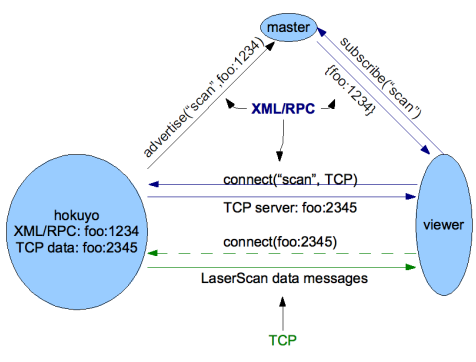
\includegraphics{figures/3_master-node-example.png}
\caption{\label{fig:master_node_example} A diagram of controlling a Hokuyo laser range-finder. Details can be found at the \href{http://www.ros.org/wiki/ROS/Technical\%20Overview}{ROS website}.}
\end{figure}

ROS uses a peer-to-peer architecture over a TCP network, allowing for
various styles of communication. The basic building block in ROS is
a \emph{node}.  Each node is a modular process with some specialized
purpose. A particular node, for example, might implement a robot's
basic motor control, or publish information from a camera.
Furthermore, these simple nodes may be combined in various ways to
form more complex nodes governing more sophisticated behaviors.  For
instance, an obstacle-avoidance node may combine information from a
robot's sensors, actuators and higher-level control architecture to
compute a maneuver.  A primary motivation of ROS is to promote code
reuse, and the modularity and platform-independence of nodes helps
serve this purpose.

\begin{wrapfigure}{r}{0.35\columnwidth}
\centering
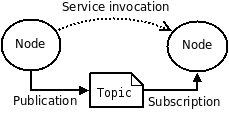
\includegraphics[width=0.3\columnwidth]{figures/3_ros_messaging.png}
\caption{\label{fig:ros_messaging}ROS messaging.}
\end{wrapfigure}

Nodes communicate with each other by publishing messages
to \emph{topics}, which are the basic message structure for
broadcasting data. Nodes publish messages to a topic as well as subscribe
to a topic to receive messages, as seen in
Figure \ref{fig:ros_messaging}\footnote{Source: http://www.ros.org/wiki/ROS/Concepts}. 
Thus topics are intended for
unidirectional, streaming communication. In general, nodes are not
aware of who they are communicating with. Instead, nodes that are
interested in data subscribe to the relevant topic; nodes that
generate data publish to the relevant topic. Figure \ref{fig:master_node_example}\footnote{Source: http://www.ros.org/wiki/ROS/Technical\%20Overview} 
provides an illustration of communication between nodes; the ``hokuyo" node 
publishes messages on the ``scan" topic and the ``viewer" node subscribes to the
``scan" topic. The two nodes are decoupled and need not know of each other.
 
Nodes that need to perform remote procedure calls, i.e. receive a
response to a request, should use \emph{services} instead. Unlike the
publish/subscribe communication paradigm that topics provide, services
allow for Remote Procedure Call (RPC) request/reply interactions which
are often required in a distributed system. Request/reply is done via
a Service, which is defined by a pair of Messages: one for the request
and one for the reply.

A complex program could potentially consist of tens or hundreds of
nodes, and these nodes need some efficient way to communicate with
each other. Thus, every program in ROS is run with a special node
called the \emph{master node}. Conceptually, this node is a
matchmaker: it is responsible for listening to node offers and
requests, and then introducing relevant nodes to each other so that
they can communicate. The master nodes provides naming and
registration services to the rest of
the \href{http://www.ros.org/wiki/Nodes}{nodes} in the ROS system. They
track publishers and subscribers
to \href{http://www.ros.org/wiki/Topics}{topics} as well
as \href{http://www.ros.org/wiki/Services}{services}. Thus the role of
the master nodes is to enable individual ROS nodes to locate one
another. Once these nodes have located each other they communicate
with each other peer-to-peer.

ROS client libraries for various programming languages,
(eg \verb/roscpp, rospy, rosjava/) exist that facilitate the
developer to program ROS nodes, publish and subscribe to topics, and
write and call services.
 
In addition to being a robot middleware system, ROS provides package
management along with an integrated build system. It also provides
tools and libraries for obtaining, building, writing, and running code
across multiple computers. Finally ROS allows for integration of
external packages, repositories and third-party software such as
OpenCV, OpenRAVE and even Player.

\subsection{ROS Quick Start with Create}
\label{sec:ros_quickstart}

The \href{http://code.google.com/p/brown-ros-pkg/}{Brown ROS package} is a set of nodes that provides basic sensing and movement functionality for the iRobot Create. This section demonstrates creating an \texttt{irobot\_create\_controller} node and writing a controller that provides a simple method to determine whether the robot's left or right bumper is pressed, as well as to set the robot's speed and rotation. This controller will rotate the Create in place until Ctrl-c is pressed.

\begin{itemize}

\item From the ROS root directory on the EeePC: \texttt{cd ros-1.0.0/pkg}\\
(Don't forget to \texttt{source rosenv} from the ROS root directory).

\item Create a ROS package for our controller:\\
\texttt{roscreate-pkg irobot\_create\_controller roscpp std\_msgs irobot\_create\_2\_1}\\
The \texttt{roscreate-pkg} command-line tool automatically creates a new ROS package called \texttt{irobot\_create\_controller} with dependencies on three other packages (\texttt{roscpp}, \texttt{std\_msgs} and \texttt{irobot\_create\_2\_1}). It generates a number of files for building the new package.

\item Create a \texttt{client.cpp} file in \texttt{irobot\_create\_controller/src} and add the following code to \texttt{client.cpp}:

\begin{verbatim}
#include <ros/ros.h>
#include <irobot_create_2_1/SensorPacket.h>
#include <geometry_msgs/Twist.h>
#include <signal.h>

ros::Publisher create_pub;
ros::Subscriber create_sub;

// Declare Ctrl-C related variables
bool endnow = false;
void stopper(int x)
{
  endnow = true;
}

// Master node calls this function everytime a new message arrives
void createListen(const irobot_create_2_1::SensorPacketConstPtr& msg)
{
  printf("Left: %d, Right: %d\n", msg->bumpLeft, msg->bumpRight);  
}

int main(int argc, char** argv) {

  // Initialize ROS
  ros::init(argc, argv, "controller");
  // Create a handle to this process node
  ros::NodeHandle n;
  // Publish messages of type geometry_msgs/Twist on topic "cmd_vel"
  create_pub = n.advertise<geometry_msgs::Twist>("cmd_vel", 1);
  // Subscribe to the "sensorPacket" topic.
  create_sub = n.subscribe("sensorPacket", 0, createListen);

  // Tell the function 'stopper' to receive all SIGINT signals	
  signal(SIGINT,stopper);

  while(!endnow)
    {
      double forward = 0.0;
      double rotate = 0.3;

      // Create and publish a Twist message
      geometry_msgs::Twist twist;
      twist.linear.x = forward; twist.linear.y = 0; twist.linear.z = 0;
      twist.angular.x = 0; twist.angular.y = 0; twist.angular.z = rotate;
      create_pub.publish(twist);

      ros::spinOnce();
    }

  // Stop the robot's movement
  geometry_msgs::Twist twist;
  twist.linear.x = 0; twist.linear.y = 0; twist.linear.z = 0;
  twist.angular.x = 0; twist.angular.y = 0; twist.angular.z = 0;
  create_pub.publish(twist);

  printf("Done.\n");
	
  return(0);
}
\end{verbatim}

The Create driver publishes a single message type, \texttt{SensorPacket.msg}, which exports all of the robot's sensory information. The message file exists in:\\ ros-1.0.0/pkg/irobot\_create\_2\_1/msg/SensorPacket.msg\\ 
For online documentation, visit the Brown ROS Create Driver \href{http://code.google.com/p/brown-ros-pkg/wiki/irobot\_create\_2\_1}{site}.

Additionally, use this \href{http://www.ros.org/wiki/ROS/Tutorials/WritingPublisherSubscriber(c\%2B\%2B)}{ROS tutorial} as a helpful resource for writing simple Publish and Subscriber nodes in C++.

\item Edit \texttt{irobot\_create\_controller/CMakeLists.txt} and add the following line to the end of the file:\\
\texttt{rosbuild add executable(client src/client.cpp)}\\
This causes an executable named \texttt{client} to be created whenever you run the command \texttt{rosmake irobot\_create\_controller}. For more information on CMake, refer to Section \ref{sec:3_cmake}, however most of the work in creating CMakeLists is done automatically by ROS.

\item Compile: \texttt{rosmake irobot\_create\_controller}

\item Turn on the Create base.

\item Run the ROS master: \texttt{roscore}

\item Run the Create driver: \texttt{rosrun irobot\_create\_2\_1 driver.py}

\item Run the controller client: \texttt{rosrun irobot\_create\_controller client}

\end{itemize}

\section{Other Middleware Packages}

There are many suitable robot middleware packages beyond Player and ROS, some of which are described in brief below.  For an excellent comparison of robot middleware, we refer the reader to the survey and analysis conducted by Huang et. al.\footnote{Huang, Olson and Moore, \textit{Lightweight Communications and Marshalling for Low Latency Interprocess Communication}, Technical Report MIT-CSAIL-TR-2009-041, 2009.}

\subsection{LCM}

\href{http://code.google.com/p/lcm/}{Lightweight Communications and Marshalling (LCM)} is ``a library for message passing and data marshalling targeted at real-time systems where high-bandwidth and low latency are critical. It provides a publish/subscribe message passing model and an XDR-style message specification language with bindings for applications in C, Java, and Python. It was originally designed and used by the \href{http://grandchallenge.mit.edu/}{MIT DARPA Urban Challenge Team} as its message passing system. LCM is designed for tightly-coupled systems connected via a dedicated local-area network. It is not intended for message passing over the Internet. LCM has been developed for soft real-time systems: its default messaging model permits dropping messages in order to minimize the latency of new messages."\footnote{code.google.com/p/lcm}

Features include:
\begin{itemize}
\item Low-latency inter-process communication
\item Efficient broadcast mechanism using UDP Multicast
\item Provides type-safe message marshaling that automatically detects most types of errors (such as version mismatches between different modules)
\item User-friendly logging and playback
\item Essentially unlimited packet size
\item No centralized ``database'' or ``hub'' -- peers communicate directly
\item No daemons
\item Supports C/C++, Java, Python, and MATLAB 
\end{itemize}

\subsection{Orocos}

The \href{http://www.orocos.org/}{Open Robot Control Software} project aims to provide a modular framework for robot and machine control.\footnote{www.orocos.org}

\subsection{YARP}

\href{http://eris.liralab.it/yarp/}{Yet Another Robot Platform} is ``an open-source framework that supports distributed computation with an eye at robot control and efficiency.  YARP supports building a robot control system as a collection of programs communicating in a peer-to-peer way, with a family of connection types that meet the diverse, sometimes contradictory, and always changing needs of advanced robotics."\footnote{eris.liralab.it/yarp}

\subsection{CARMEN}

\href{http://carmen.sourceforge.net}{The Carnegie Mellon Robot Navigation Toolkit (CARMEN)} is ``an open-source collection of software for mobile robot control. CARMEN is modular software designed to provide basic navigation primitives including: base and sensor control, logging, obstacle avoidance, localization, path planning, and mapping."\footnote{carmen.sourceforge.net}

\subsection{Microsoft Robotics Studio}

\href{http://msdn.microsoft.com/en-us/robotics/default.aspx}{Microsoft Robotics Studio} is ``a Windows-based environment for hobbyist, academic and commercial developers to create robotics applications for a variety of hardware platforms."\footnote{msdn.microsoft.com/en-us/robotics}

\subsection{JAUS}

Joint Architecture for Unmanned Systems ``was originally an initiative by the US Department of Defense to develop an open architecture for the domain of unmanned systems.''\footnote{en.wikipedia.org/wiki/JAUS}

\section{Version Control using Subversion}

Version control systems are a class of software that keeps track of revisions to files as they are made and edited. One popular open source version control system is \href{http://subversion.tigris.org/}{Subversion}. From \texttt{man svn}:

\begin{quote}
Subversion is a version control system, which allows you to keep old versions of files and directories (usually source code), keep a log of who, when, and why changes occurred, etc., like CVS, RCS or SCCS. Subversion keeps a single copy of the master sources. This copy is called the source ``repository''; it contains all the information to permit extracting previous versions of those files at any time.
\end{quote}

CS148 requires students to use Subversion to submit the code for finished assignments. In addition to helping students keep track of the revisions they make for their source code, Subversion facilitates collaborative development on source code. Anyone in a project group can check out code, modify it, and commit their changes to a common repository. A student can then update the code they are working on with their changes without having to trade whole files back and forth. Additionally, code can be checked out directly to one of the class robots, allowing for greater portability when switching between robots.

Our aim is for students who have not used a version control system before will gain familiarity with version control and learn how to use Subversion to guide their group's workflow, while those who have will be able to start working with Subversion right away. \href{http://svnbook.red-bean.com/}{Version Control with Subversion} is a very comprehensive book freely available, which gives extensive documentation on Subversion.

\subsection{Repository Setup by Admin}

The course staff is responsible for setting up a Subversion repository for each group. We want students to be able to check out code directly onto the EeePCs. Because Subversion repositories cannot be accessed directly via SSH, the course staff runs a network service (\textit{svnserve}) to allow for this. This requires an additional machine that both runs the service and hosts the repositories, as well as a wireless network that the robot EeePCs can connect to. \textit{svnserve} is a small and lightweight server program; it is advantageous because there is no need to create system accounts on the server and passwords are not passed over the network. However by default, \textit{svnserve} does not provide encryption or logging, and the server stores clear text passwords. Overall, \textit{svnserve} is easy to setup and suits our purposes. For an overview and comparison of other svn server configurations options, please see Chapter 6 of \href{http://svnbook.red-bean.com/en/1.5/index.html}{``Version Control with Subversion"}, which is available online.

The following are instructions for an admin to create a student group repository, set up the repository structure, run \textit{svnserve}, and test checking out. All of this should be done on another machine connected to the wireless network. In this example, COURSE\_HOME is the root of your course directory and ``148student" is the name of the student repository.

\begin{itemize}

\item Create a student repository.\\
\texttt{cd COURSE\_HOME}\\
\texttt{mkdir svn/148student}\\
\texttt{svnadmin create COURSE\_HOME/svn/148student}

\item Create a repository structure with /tags, /trunk and /branches directories inside the repository. To do this, we first locally checkout the newly created repository, create each directory, commit and cleanup.\\
\texttt{cd COURSE\_HOME}\\
\texttt{svn checkout file://COURSE\_HOME/svn/148student tmp}\\
\texttt{cd tmp}\\
\texttt{mkdir tags trunk branches}\\
\texttt{svn add tags trunk branches}\\
\texttt{svn commit -m "Created initial Subversion repository structure"}\\
\texttt{cd ..}\\
\texttt{rm -rf tmp}

\item In \texttt{svn/148student/conf/svnserve.conf}, uncomment/edit the following lines:\\
\texttt{anon-access = none}\\
\texttt{auth-access = write}\\
\texttt{password-db = passwd}\\
\texttt{authz-db = authz}\\
\texttt{realm = 148student repository}

\item Add the following lines to \texttt{svn/148student/conf/authz}:\\
\texttt{[groups]}\\
\texttt{students = 148student}\\
\texttt{[/]}\\
\texttt{@students = rw}

\item Set the user password. In \texttt{svn/148student/conf/passwd}:\\
\texttt{[users]}\\
\texttt{148student = MyPassword}

\item To disable password caching, in \texttt{~/.subversion/config} on each EeePC, add/uncomment the line: \texttt{store-passwords = no}\\
By default, Subversion caches passwords in plain text on disk. Since students will most likely share EeePCs and have access to every EeePC, it is necessary to disable password caching on the EeePC so students cannot check out each other's code.

\item Run svnserve as a standalone daemon process:\\
\texttt{svnserve -d}

\item Test checking out from an EeePC connected to a wireless network.\\
\texttt{svn checkout svn://<IP>/148student/trunk <dirname>}\\
$<$IP$>$ should be the IP address of the computer running svnserve.

\item For more resources, read the manpages for \texttt{svnadmin}, the administrative command for Subversion. Also refer to Chapters 5 and 6 of \href{http://svnbook.red-bean.com/en/1.5/index.html}{``Version Control with Subversion"}.

\end{itemize}

\subsection{Repository Use by Students}

\subsubsection{Concepts}

Subversion may be thought of as a file versioning system that sits on top of a filesystem. With it, one can take a set of files, apply changes to them, commit the new changes, and continue working. At any point in time, one can revisit his or her files as they were at an earlier revision. What follows is a brief glossary of terms.

\begin{itemize}
\item Repository: a central location where your project resides.
\item Working copy: a file tree you have checked out from the repository.
\item Revision: every time you commit code to your repository, a new revision is created and given a number. You can refer to the repository as it was at a specific commit using that commit's revision number.
\item Trunk: a file tree that contains your main body of code.
\item Tags: a tag is a special name that you give to some snapshot of code in the repository. In Subversion, this is a copy of some file tree that you give a special name in the top-level directory tags.
\item Branches: a branch is a section of material that is being worked on in separately from other code in order to isolate one set of changes from others. In Subversion, this is a copy of some file tree that you have given a special name in the top-level directory branches. 
\end{itemize}

When accessing the repository for the first time, students will be prompted for a username/password pair. To specify a particular username to svn, use the --username argument.

\subsubsection{The Repository Structure}

At their top level of a student's Subversion repository are the directories \texttt{trunk}, \texttt{tags}, and \texttt{branches}. Typically \texttt{trunk} should be used for whatever is currently being worked on, while \texttt{tags} and \texttt{branches} hold tags and branches of the work, respectively.

\subsubsection{Subversion commands}

The command-line Subversion client is \texttt{svn}. Invocations of the client use this syntax: \\

\texttt{svn <action> [arguments]}\\

\begin{itemize}
\item Browsing the repository

To examine the contents of the repository before checking anything out: \texttt{svn ls svn://host/groupname/svn}\\

svn has analogues to the Unix \texttt{ls}, \texttt{cat}, \texttt{mv}, \texttt{rm}, and cp commands that can all work directly on the repository. 

\item Checking out

To get started, one should check out a new working copy of a repository. This only needs to happen once, unless for some reason multiple working copies of your code exist. To check out your trunk directory, run:

\texttt{svn checkout svn://host/groupname/trunk <dirname>}

One should end up with a new directory with the name $<$dirname$>$ where the command was run. One can treat this directory as if it were any other and develop projects in it. Future example commands with svn will assume that the commands are run from within the working copy that was just checked out. As you start out, you should see using \texttt{svn ls} that you have a few \texttt{branches} in branches and nothing else in any of the other top-level directories. 

\item Updating

It is important to update a working copy of the repository whenever another group member commits any of their work. To update a working copy, run:\\

\texttt{svn update}\\

This will download any changes that other group members have made and then apply them to the current working copy. If there are conflicts between changes made in the current working copy and changes that have been committed to the repository, they will need to be resolved.

To update to an older version of the repository:

\texttt{svn update -r <revision>}

See svn help update for information about what $<$revision$>$ might be. If svn update is ran to look at old versions, it is important to svn update again later to keep updated with the latest repository version

\item Examining the state of a working copy

To see what changes have been made to a current working copy relative to what files in the repository, run:

\texttt{svn status}

See \texttt{svn help status} for information about what the output means. It is good practice to run this before committing, in order to see what changes have been made.

To see specific changes made, use \texttt{svn diff}. This can be run with a specific file argument to display the changes made to that file.

\item Manipulating files in a working copy

The \texttt{svn cp}, \texttt{svn mv}, and \texttt{svn rm} commands mentioned above may be used directly on a repository, and they should also be used to manipulate files in a working copy. To rename:

\texttt{svn mv <file1> <file2>}

This will rename the file in a manner that Subversion is aware of it and will track it when committing this change.

\item Committing changes

Committing work to the group repository is known as ``checking in''. Always run \texttt{svn update} before a commit.

To mark the new files that should be committed as ``added'' before committing them to the repository, use \texttt{svn add}.

\texttt{svn add <file1> [file2] ...}

View the changed status of files with \texttt{svn status}.

Once the new files have been added as files to commit, run:

\texttt{svn commit}

An editor will pop up asking for a message describing the commit. It is good practice to write something informative, maybe even detailing what semantic changes were made to each file, save the message, and then exit the editor.

\item Resolving conflicts

It does happen that, while working on one section of a project, someone else will commit something that overlaps with what is being worked on in your working repository. One may resolve the conflict immediately using an interactive prompt, or will need to look at the files with conflicting sections, edit them appropriately, and then mark them with:

\texttt{svn resolved <file1> [file2]}

\item Other helpful commands:
\noindent \texttt{svn help <action>} to get usage for a specific action.\\
\noindent \texttt{svn help} lists all of the Subversion commands.\\
\noindent \texttt{svn revert} to undo changes to a file and reset it to a just-checked-out state.
\noindent \texttt{svn log} to view a history of commits and their messages. 

\item Merging from branches

We provide students with skeleton code for the first assignment. Before beginning work on the first assignment, students should pull its respective skeleton code into their group's trunk. Students should then proceed to work in their own trunk.

Conceptually, what you need to do is merge the code in the branch onto whatever is currently in your trunk. This is very easy for assignment 1, as you are starting with an empty trunk. Once you have checked out your trunk (with \texttt{svn checkout}), the command to do this is:

\texttt{svn merge svn://host/groupname/branches/asgn1\_skel}

You then must commit the merged changes with \texttt{svn add} and \texttt{svn commit}.

See \texttt{svn merge help} for further explanation of this command. Once again, the section of the Subversion book on branching and merging gives a comprehensive treatment of the subject.

\end{itemize}

\subsection{Assignment Submissions}

To submit assignments, we expect students to ``tag" their current working trunk directory; the course staff then checks out the current assignment folder within each group's tags directory. Remember, tagging is simply taking a snapshot in the repository. Students should follow the instructions below to submit for an Assignment 0:\\
\texttt{svn add <files>}\\
\texttt{svn commit -m "Tagging assignment 0"}\\
\texttt{svn cp svn://host/groupname/trunk svn://host/groupname/tags/asgn0}\\

\section{Building with CMake}

\label{sec:3_cmake}

\href{http://www.cmake.org/}{CMake} is an open-source build system that we encourage students to use as an alternative option to the make build system. CMake tries to get around some of make's shortcomings (such as whitespace-sensitivity) by providing an easy way of declaring how your project is compiled. From the cmake manpage:

\begin{quote}
CMake is a cross-platform build system generator. Projects specify their build process with platform-independent CMake listfiles included in each directory of a source tree with the name CMakeLists.txt. Users build a project by using CMake to generate a build system for a native tool on their platform.
\end{quote}

Please refer to CMake's \href{http://www.cmake.org/cmake/help/cmake2.6docs.html}{documentation} as an additional resource.

\noindent
CMake builds makefiles by default. Below is a ``Hello World" example with CMake:

\begin{itemize}
\item In an empty directory, save the following as \texttt{hello.cpp}:
\begin{verbatim}
#include <stdio.h>
int main() {
  printf("hello world.\n");
  return 0;
}
\end{verbatim}

\item Save the following as \texttt{CMakeLists.txt}:
\begin{verbatim}
cmake_minimum_required(VERSION 2.0)
project(MyProject)
add_executable(hello hello.cpp)
\end{verbatim}

\item Run: \texttt{cmake .}\\
This reads your CMakeLists.txt and builds your makefiles. In addition to Makefile (the actual makefile), CMake generates CMakeCache.txt, cmake\_install.cmake, and the directory CMakeFiles. These can be ignored.

\item Run: \texttt{make}\\
This reads the makefiles written by cmake and builds your project. The next time you edit any of your existing files, you do not have to run \texttt{cmake .} again; you only need to \texttt{make} again to recompile the project. However if you add or remove files from your project or decide to change how it is built (such as by changing your compiler options or adding a library dependency), you do have to run \texttt{cmake .} again to regenerate a Makefile.

\end{itemize}

Player is not dependent on CMake, however ROS uses CMake as their core build system. If you use ROS you will not have to worry about creating CMakeLists.txt files because this is automatically done for you, however you will have to add lines to CMakeLists.txt for adding new libraries or executables to your ROS package.

\newpage
